\subsection{Spectral Analysis of C-elegans}
\label{section: Spectral Analysis}

\paragraph{Note}
There are 4 types of membrane regenerative potentials:
\begin{itemize}
  \item Action potential
  \item Graded potential
  \item Intrinsic oscillation
  \item Plateau potential
\end{itemize}

The following papers disagree on the type of membrane potential that the neurons of C. elegans use: 
\cite{mellem_action_2008}, \cite{lockery_first_2009}, \cite{lockery_quest_2009}.
The last two articles are written by the same people: Shawn Lockery (University of Oregon) and Miriam Goodman (Stanford University).

\paragraph{Hodgkin-Huxley Equation} is used to predict the quantitative behavior of a model nerve under a variety of conditions which corresponded to those in actual
experiments. Their experiments show that the neuron cell membrane potential during an acitivity will rise from $-65mV$ to above $+40mV$ at the peak. This phenonmenon is
explained by the changing permeability of different ions according to their voltage clamp experiment, which turns out to be an accurate electric model of neuron
communication. 

\begin{figure}[h!]
  \centering
  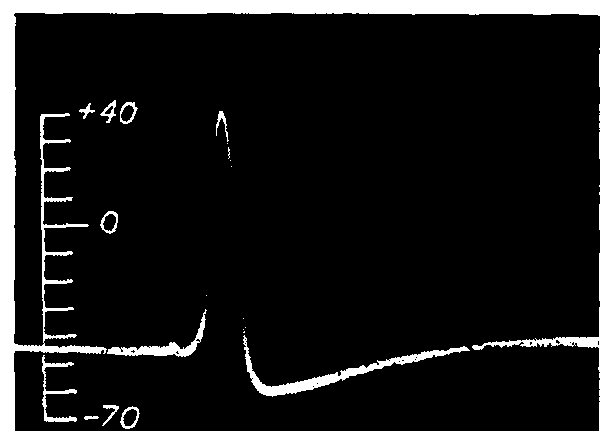
\includegraphics[width=0.5\textwidth]{graphics/ActionPotential}
  \label{fig:action_potential}
  \caption{Action potential and resting potential recorded between inside and outside of axon with capillary filled with sea water. The sea water outside is treated as
zero potential  \cite{Hodgkin_quantitative_1990} }
\end{figure}

% picture from http://www.helcohi.com/sse/body/nervous.html
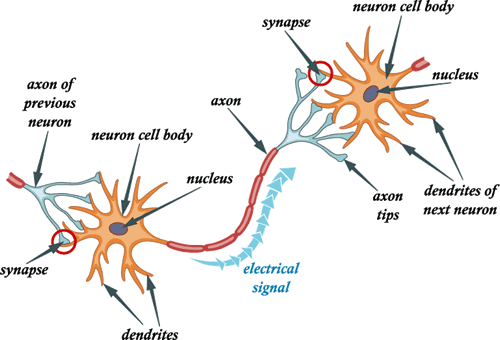
\includegraphics[scale=0.8]{graphics/NeuronSignal}

The following is my summery for the phases that the excitation of neurons goes through:
\begin{enumerate}
  \item The firing threshold is reached. Action potential jumps high. There is influx of sodium ion through the ion channel.
  \item $Na^{+}$ ion causes the membrane to be positively charged. Potassium ion starts to leave the cell(inhibitory factor).
  \item Reaches peak in action potential. Sodium channels becomes refractory, and no more sodium ion is allowed to enter.
  \item Repolarizing phase, when sodium ion channel still in its refractory phase, while potassium ions continues to leave the cell.
  \item Potassium channels close. Sodium channel ends the refractory phase and reset to resting state.
  \item Diffusion of extracellular potassium from cell causes in very slight increase in membrane voltage. (before resting, the cell is in 
	\textbf{hyper-polarizing state}, the cell is not available for the next stimulation.
\end{enumerate}

An illustration of various phases:

% from http://en.wikipedia.org/wiki/Refractory_period_(physiology)
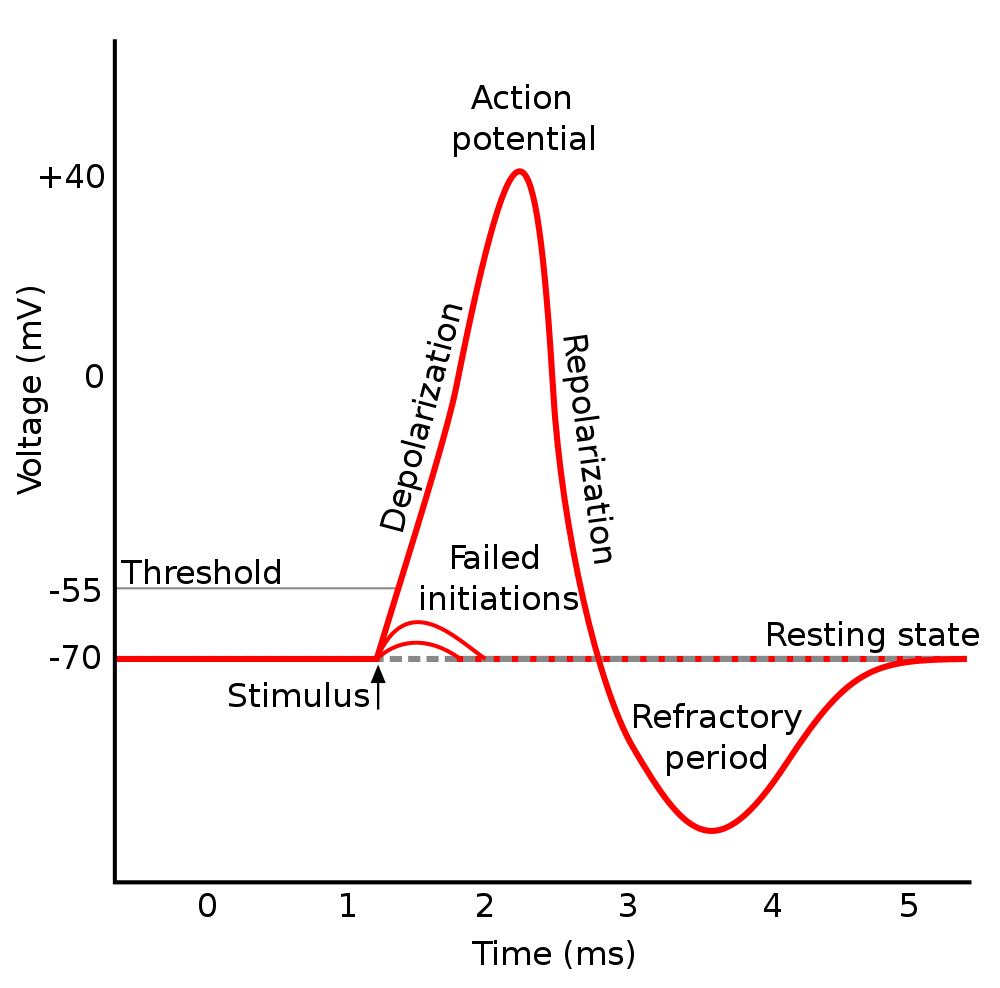
\includegraphics[scale=0.3]{graphics/ActionPotential2}

\subsubsection{Mathematical model}

\paragraph{Model for single cell:}
$$ C_m \frac{dV_m}{dt} + I_{ion} = I. $$
Where $C_m$ denotes membrane capacitance per unit area; $V_m$ the displacement of the membrane potential from its resting value (depolarization
negative); $t$ the time, $I_{ion}$ the net ion current flowing accross the
membrane (inward current positive), and $I$ the total ion current density (inward current positive).

The $I_{ion}$ can be further split into 3 components:
$$ I_{ion} = I_{Na} + I_{K} + I_{l}, \\
\begin{cases}
  I_{Na} = g_{Na} (E - E_{Na}), \\
  I_{K} = g_{K} (E - E_{K}), \\
  I_{l} = {\bar{g}}_{l}.
\end{cases}
$$
The leakage current $I_{l}$ is caused by other ions such as $Cl^{-}$.
$E_{Na}$ and $E_{K}$ are the equilibrium potentials for $Na^{+}$ and $K^{+}$.

The movement of ions is proportional to conductance times driving force.
Let
$$
\begin{cases}
  V = E - E_r, \\
  V_{Na} = E_{Na} - E_r, \\
  V_{K} = E_{K} - E_r, \\
  V_{l} = E_{l} - E_r.
\end{cases}
$$
The $E$s can be replaced by $V$s with respect to resting potential.

Ion channels for different ions contains many gates. If all gates are in permissive state, the channel is considered to be open, and ions are able to go through. The
probability of a gate being in permissive state depends on the current value of the membrane voltage. HH model the gates as their probability of being in permissive
state, ie. $m$, $n$, and $h$. The model specifies the number of gates each ion channel has:

$$
I_{ion} = {\bar{g}}_{Na} m^3 h (V - V_{Na}) + {\bar{g}}_K n^4 (V - V_K) + {\bar{g}}_l (V - Vl),
$$

where
$$ \frac{dn}{dt} = \alpha_n (1 - n) - \beta_n n, $$
$$ \frac{dm}{dt} = \alpha_m (1 - m) - \beta_m m, $$
$$ \frac{dh}{dt} = \alpha_h (1 - h) - \beta_h h. $$

and

$$ \alpha_n = \frac{0.01(V + 10)}{exp \frac{V + 10}{10} - 1}, $$
$$ \beta_n = 0.125 exp \frac{V}{80}, $$
$$ \alpha_m = \frac{0.1(V + 25)}{exp \frac{V + 25}{10} - 1}, $$
$$ \beta_m = 4 exp \frac{V}{18}, $$
$$ \alpha_h = 0.07 exp \frac{V}{20} $$
$$ \beta_h = \frac{1}{exp \frac{V + 30}{10} + 1}. $$

The above number and type of gates for each channel was determined using a trial-and-error method to find the order of gates to achieve the sigmoidal conductance found
from previous results. The best match is the power of 4. The rate constants are obtained by fitting conductance data:

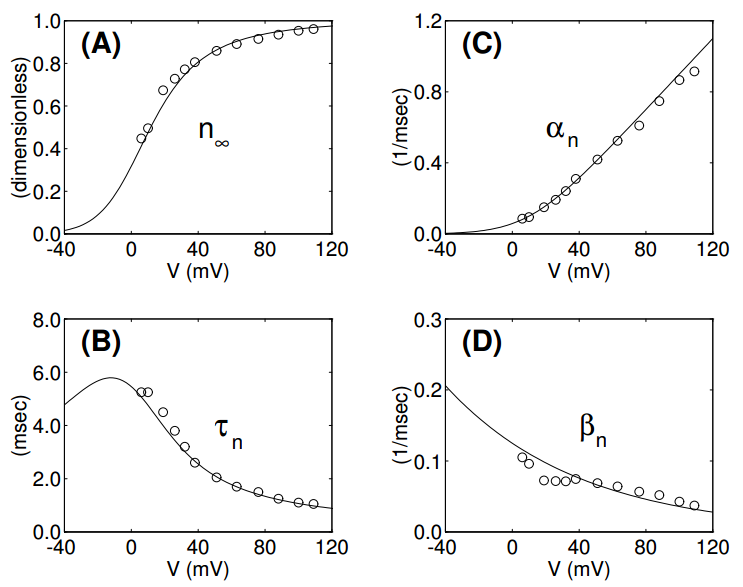
\includegraphics[scale=0.6]{graphics/RateConstants}

\subsubsection{Simplification of HH Equation}
FitzHugh-Nagumo Model:
$$ \dot{V} = V - \frac{V^3}{3} - W + I $$
$$ \dot{W} = 0.08(V + 0.7 - 0.8W) $$



